%%
%% This is file `sample-sigconf.tex',
%% generated with the docstrip utility.
%%
%% The original source files were:
%%
%% samples.dtx  (with options: `all,proceedings,bibtex,sigconf')
%% 
%% IMPORTANT NOTICE:
%% 
%% For the copyright see the source file.
%% 
%% Any modified versions of this file must be renamed
%% with new filenames distinct from sample-sigconf.tex.
%% 
%% For distribution of the original source see the terms
%% for copying and modification in the file samples.dtx.
%% 
%% This generated file may be distributed as long as the
%% original source files, as listed above, are part of the
%% same distribution. (The sources need not necessarily be
%% in the same archive or directory.)
%%
%%
%% Commands for TeXCount
%TC:macro \cite [option:text,text]
%TC:macro \citep [option:text,text]
%TC:macro \citet [option:text,text]
%TC:envir table 0 1
%TC:envir table* 0 1
%TC:envir tabular [ignore] word
%TC:envir displaymath 0 word
%TC:envir math 0 word
%TC:envir comment 0 0
%%
%% The first command in your LaTeX source must be the \documentclass
%% command.
%%
%% For submission and review of your manuscript please change the
%% command to \documentclass[manuscript, screen, review]{acmart}.
%%
%% When submitting camera ready or to TAPS, please change the command
%% to \documentclass[sigconf]{acmart} or whichever template is required
%% for your publication.
%%
%%
% \documentclass[sigconf]{acmart}
\documentclass[sigconf, anonymous, review]{acmart}
%%
%% \BibTeX command to typeset BibTeX logo in the docs
\AtBeginDocument{%
  \providecommand\BibTeX{{%
    Bib\TeX}}}

%% Rights management information.  This information is sent to you
%% when you complete the rights form.  These commands have SAMPLE
%% values in them; it is your responsibility as an author to replace
%% the commands and values with those provided to you when you
%% complete the rights form.
\setcopyright{acmlicensed}
\copyrightyear{2018}
\acmYear{2018}
\acmDOI{XXXXXXX.XXXXXXX}
%% These commands are for a PROCEEDINGS abstract or paper.
\acmConference[Conference acronym 'XX]{Make sure to enter the correct
  conference title from your rights confirmation email}{June 03--05,
  2018}{Woodstock, NY}
%%
%%  Uncomment \acmBooktitle if the title of the proceedings is different
%%  from ``Proceedings of ...''!
%%
%%\acmBooktitle{Woodstock '18: ACM Symposium on Neural Gaze Detection,
%%  June 03--05, 2018, Woodstock, NY}
\acmISBN{978-1-4503-XXXX-X/2018/06}


%%
%% Submission ID.
%% Use this when submitting an article to a sponsored event. You'll
%% receive a unique submission ID from the organizers
%% of the event, and this ID should be used as the parameter to this command.
%%\acmSubmissionID{123-A56-BU3}

%%
%% For managing citations, it is recommended to use bibliography
%% files in BibTeX format.
%%
%% You can then either use BibTeX with the ACM-Reference-Format style,
%% or BibLaTeX with the acmnumeric or acmauthoryear sytles, that include
%% support for advanced citation of software artefact from the
%% biblatex-software package, also separately available on CTAN.
%%
%% Look at the sample-*-biblatex.tex files for templates showcasing
%% the biblatex styles.
%%

%%
%% The majority of ACM publications use numbered citations and
%% references.  The command \citestyle{authoryear} switches to the
%% "author year" style.
%%
%% If you are preparing content for an event
%% sponsored by ACM SIGGRAPH, you must use the "author year" style of
%% citations and references.
%% Uncommenting
%% the next command will enable that style.
%%\citestyle{acmauthoryear}


%%
%% end of the preamble, start of the body of the document source.
\begin{document}

%%
%% The "title" command has an optional parameter,
%% allowing the author to define a "short title" to be used in page headers.
\title{The Name of the Title Is Hope}

%%
%% The "author" command and its associated commands are used to define
%% the authors and their affiliations.
%% Of note is the shared affiliation of the first two authors, and the
%% "authornote" and "authornotemark" commands
%% used to denote shared contribution to the research.
\author{Ben Trovato}
\authornote{Both authors contributed equally to this research.}
\email{trovato@corporation.com}
\orcid{1234-5678-9012}
\author{G.K.M. Tobin}
\authornotemark[1]
\email{webmaster@marysville-ohio.com}
\affiliation{%
  \institution{Institute for Clarity in Documentation}
  \city{Dublin}
  \state{Ohio}
  \country{USA}
}

\author{Lars Th{\o}rv{\"a}ld}
\affiliation{%
  \institution{The Th{\o}rv{\"a}ld Group}
  \city{Hekla}
  \country{Iceland}}
\email{larst@affiliation.org}

\author{Valerie B\'eranger}
\affiliation{%
  \institution{Inria Paris-Rocquencourt}
  \city{Rocquencourt}
  \country{France}
}

\author{Aparna Patel}
\affiliation{%
 \institution{Rajiv Gandhi University}
 \city{Doimukh}
 \state{Arunachal Pradesh}
 \country{India}}

\author{Huifen Chan}
\affiliation{%
  \institution{Tsinghua University}
  \city{Haidian Qu}
  \state{Beijing Shi}
  \country{China}}

\author{Charles Palmer}
\affiliation{%
  \institution{Palmer Research Laboratories}
  \city{San Antonio}
  \state{Texas}
  \country{USA}}
\email{cpalmer@prl.com}

\author{John Smith}
\affiliation{%
  \institution{The Th{\o}rv{\"a}ld Group}
  \city{Hekla}
  \country{Iceland}}
\email{jsmith@affiliation.org}

\author{Julius P. Kumquat}
\affiliation{%
  \institution{The Kumquat Consortium}
  \city{New York}
  \country{USA}}
\email{jpkumquat@consortium.net}

%%
%% By default, the full list of authors will be used in the page
%% headers. Often, this list is too long, and will overlap
%% other information printed in the page headers. This command allows
%% the author to define a more concise list
%% of authors' names for this purpose.
\renewcommand{\shortauthors}{Trovato et al.}

%%
%% The abstract is a short summary of the work to be presented in the
%% article.
\begin{abstract}
  A clear and well-documented \LaTeX\ document is presented as an
  article formatted for publication by ACM in a conference proceedings
  or journal publication. Based on the ``acmart'' document class, this
  article presents and explains many of the common variations, as well
  as many of the formatting elements an author may use in the
  preparation of the documentation of their work.
\end{abstract}

%%
%% The code below is generated by the tool at http://dl.acm.org/ccs.cfm.
%% Please copy and paste the code instead of the example below.
%%
\begin{CCSXML}
<ccs2012>
 <concept>
  <concept_id>00000000.0000000.0000000</concept_id>
  <concept_desc>Do Not Use This Code, Generate the Correct Terms for Your Paper</concept_desc>
  <concept_significance>500</concept_significance>
 </concept>
 <concept>
  <concept_id>00000000.00000000.00000000</concept_id>
  <concept_desc>Do Not Use This Code, Generate the Correct Terms for Your Paper</concept_desc>
  <concept_significance>300</concept_significance>
 </concept>
 <concept>
  <concept_id>00000000.00000000.00000000</concept_id>
  <concept_desc>Do Not Use This Code, Generate the Correct Terms for Your Paper</concept_desc>
  <concept_significance>100</concept_significance>
 </concept>
 <concept>
  <concept_id>00000000.00000000.00000000</concept_id>
  <concept_desc>Do Not Use This Code, Generate the Correct Terms for Your Paper</concept_desc>
  <concept_significance>100</concept_significance>
 </concept>
</ccs2012>
\end{CCSXML}

\ccsdesc[500]{Do Not Use This Code~Generate the Correct Terms for Your Paper}
\ccsdesc[300]{Do Not Use This Code~Generate the Correct Terms for Your Paper}
\ccsdesc{Do Not Use This Code~Generate the Correct Terms for Your Paper}
\ccsdesc[100]{Do Not Use This Code~Generate the Correct Terms for Your Paper}

%%
%% Keywords. The author(s) should pick words that accurately describe
%% the work being presented. Separate the keywords with commas.
\keywords{Do, Not, Use, This, Code, Put, the, Correct, Terms, for,
  Your, Paper}
%% A "teaser" image appears between the author and affiliation
%% information and the body of the document, and typically spans the
%% page.


\received{20 February 2007}
\received[revised]{12 March 2009}
\received[accepted]{5 June 2009}

%%
%% This command processes the author and affiliation and title
%% information and builds the first part of the formatted document.

\maketitle

\section{Introduction}
TBD

\section{Method}

We propose a method that utilizes \emph{seed graphs} to anchor future question generation instead of relying on static datapoints that are susceptible to memorization or data contamination. Because each evaluation round renders a fresh QA pair from each graph, no fixed test item can be leaked ahead of time, yet all rounds remain semantically comparable via the common anchors.

\subsection{Seed Graphs}

At evaluation round $t$, we maintain a set $\mathcal{S}_t = \{ G_1^{(t)}, \ldots, G_{n_t}^{(t)} \}$ of seed graphs. Each graph encodes the evidence trail (e.g., queries, retrieved documents, answer node) for a distinct information need. To support evolving information, graphs are constructed at evaluation time.

\subsection{QA Generation}

The generation function $\text{Gen}$ takes a seed graph $G_i^{(t)}$, a random seed $r_{i,t} \sim \mathcal{R}$, and a fixed generation configuration to produce one QA pair:
\begin{equation}
    (q_{i,t}, a_{i,t}) = \text{Gen}(G_i^{(t)}; r_{i,t}, \theta)
\end{equation}

Here, $\text{Gen}$ is an LLM-based generator that bundles a frozen prompt template and fixed decoding settings (e.g., temperature, top-$p$, stop tokens). $r_{i,t}$ is an i.i.d.\ sample from randomness source $\mathcal{R}$, introducing per-sample stochasticity. Holding $\theta$ constant and varying only $r_{i,t}$ ensures that each system sees independent but identically distributed QA samples.

\subsection{Distributional Consistency}

Sampling an independent seed $r_{i,t} \sim \mathcal{R}$ for each graph yields the per-graph distribution:
\begin{equation}
    \mathcal{P}_{i,t} = \text{Dist}(\text{Gen}(G_i^{(t)}; r, \theta))
\end{equation}

Because seeds are independent across graphs, the round-$t$ dataset 
$D_t = \{ (q_{1,t}, a_{1,t}), \ldots, (q_{n_t,t}, a_{n_t,t}) \}$ 
is an i.i.d.\ sample from the product measure:
\begin{equation}
    \mathcal{P}_t = \prod_{i=1}^{n_t} \mathcal{P}_{i,t}
\end{equation}

For a model $M$ under evaluation, let $\text{score}((q, a), M)$ be any per-question metric (e.g., exact match, F1, log-loss). The aggregate dataset score is defined as:
\begin{equation}
    \text{Agg}(D_t, M) = \frac{1}{n_t} \sum_{i=1}^{n_t} \text{score}((q_{i,t}, a_{i,t}), M)
\end{equation}

By linearity of expectation and independence of $(q_{i,t}, a_{i,t}) \sim \mathcal{P}_{i,t}$:
\begin{equation}
    \mathbb{E}_{D_t \sim \mathcal{P}_t}[\text{Agg}(D_t, M)] 
    = \frac{1}{n_t} \sum_{i=1}^{n_t} \mathbb{E}_{(q,a) \sim \mathcal{P}_{i,t}}[\text{score}((q,a), M)]
\end{equation}

This shows that the expected accuracy is simply the average of the per-graph expectations—so every seed graph contributes equally.

\subsection{Collision Bound}

Assume for every seed graph $G_i^{(t)}$, the generator can produce $K$ distinct question–answer pairs:
\[
\mathcal{C}_{i,t} = \{ (q, a) \in \mathcal{P}_{i,t} \mid \Pr((q, a)) > 0 \}, \quad |\mathcal{C}_{i,t}| = K
\]

To characterize overlap across rounds $u < v$, define:
\[
J_{i,u,v} = |\mathcal{C}_{i,u} \cap \mathcal{C}_{i,v}|, \quad J_{\max} = \max_{u < v} J_{i,u,v}
\]

Because answers and evidence evolve over time, $J_{\max}$ tends to remain small for fast-changing topics.

\paragraph{Collision Probability.} Sampling one QA pair per round, the probability that seed graph $i$ produces the same QA pair twice within $t$ rounds satisfies:
\begin{equation}
    \Pr[\text{collision within } t] \leq \frac{t(t-1)}{2K^2} J_{\max}
\end{equation}

\paragraph{Collision Control.} To guarantee that this probability is at most $\delta \in (0,1)$, it suffices to choose $K$ such that:
\begin{equation}
    K \geq \sqrt{ \frac{t(t-1)}{2\delta} J_{\max} }
\end{equation}

Equation (7) captures key trade-offs:
\begin{itemize}
    \item Larger $K$ (richer candidate pool) reduces collision probability for fixed $t$.
    \item Fewer evaluation rounds $t$ allow a smaller $K$ for the same error tolerance $\delta$.
    \item Smaller $J_{\max}$ (i.e., greater semantic drift) reduces required $K$.
\end{itemize}

Because each seed graph is rebuilt from fresh evidence each round, its candidate set changes, helping keep $J_{\max}$ small. Equation (6) quantifies the collision risk, while Equation (7) provides a tunable design guideline for selecting $K$.

\subsection{Cross-Round Reporting and Compatibility}

Because each round rebuilds the seed graph set $\mathcal{S}_t$, the underlying distribution 
$\mathcal{P}_t = \prod_i \mathcal{P}_{i,t}$ may drift over time, especially for evolving topics. Consequently, raw accuracies from different rounds may not be directly comparable. We offer two strategies:

\paragraph{i) Snapshot Evaluation.} Fix a reference round $t^\ast$ and freeze its seed graphs $\mathcal{S}_{t^\ast}$. All systems are then evaluated on the same dataset $D_{t^\ast}$, ensuring identical test conditions.

\paragraph{ii) Macro-Averaged Score.} For longitudinal tracking, aggregate performance across a window $\{t_1, \ldots, t_T\}$ (e.g., most recent $T$ rounds) using:
\begin{equation}
    \text{Score}_{\text{macro}} = \frac{1}{T} \sum_{j=1}^{T} \text{Agg}(D_{t_j}, M)
\end{equation}

Each $D_{t_j}$ is i.i.d.\ from its own $\mathcal{P}_{t_j}$, so Eq.\ (8) summarizes average effectiveness under the benchmark’s natural evolution, without letting any single round dominate.

\section{Results}

\begin{figure}[htbp]
    \centering
    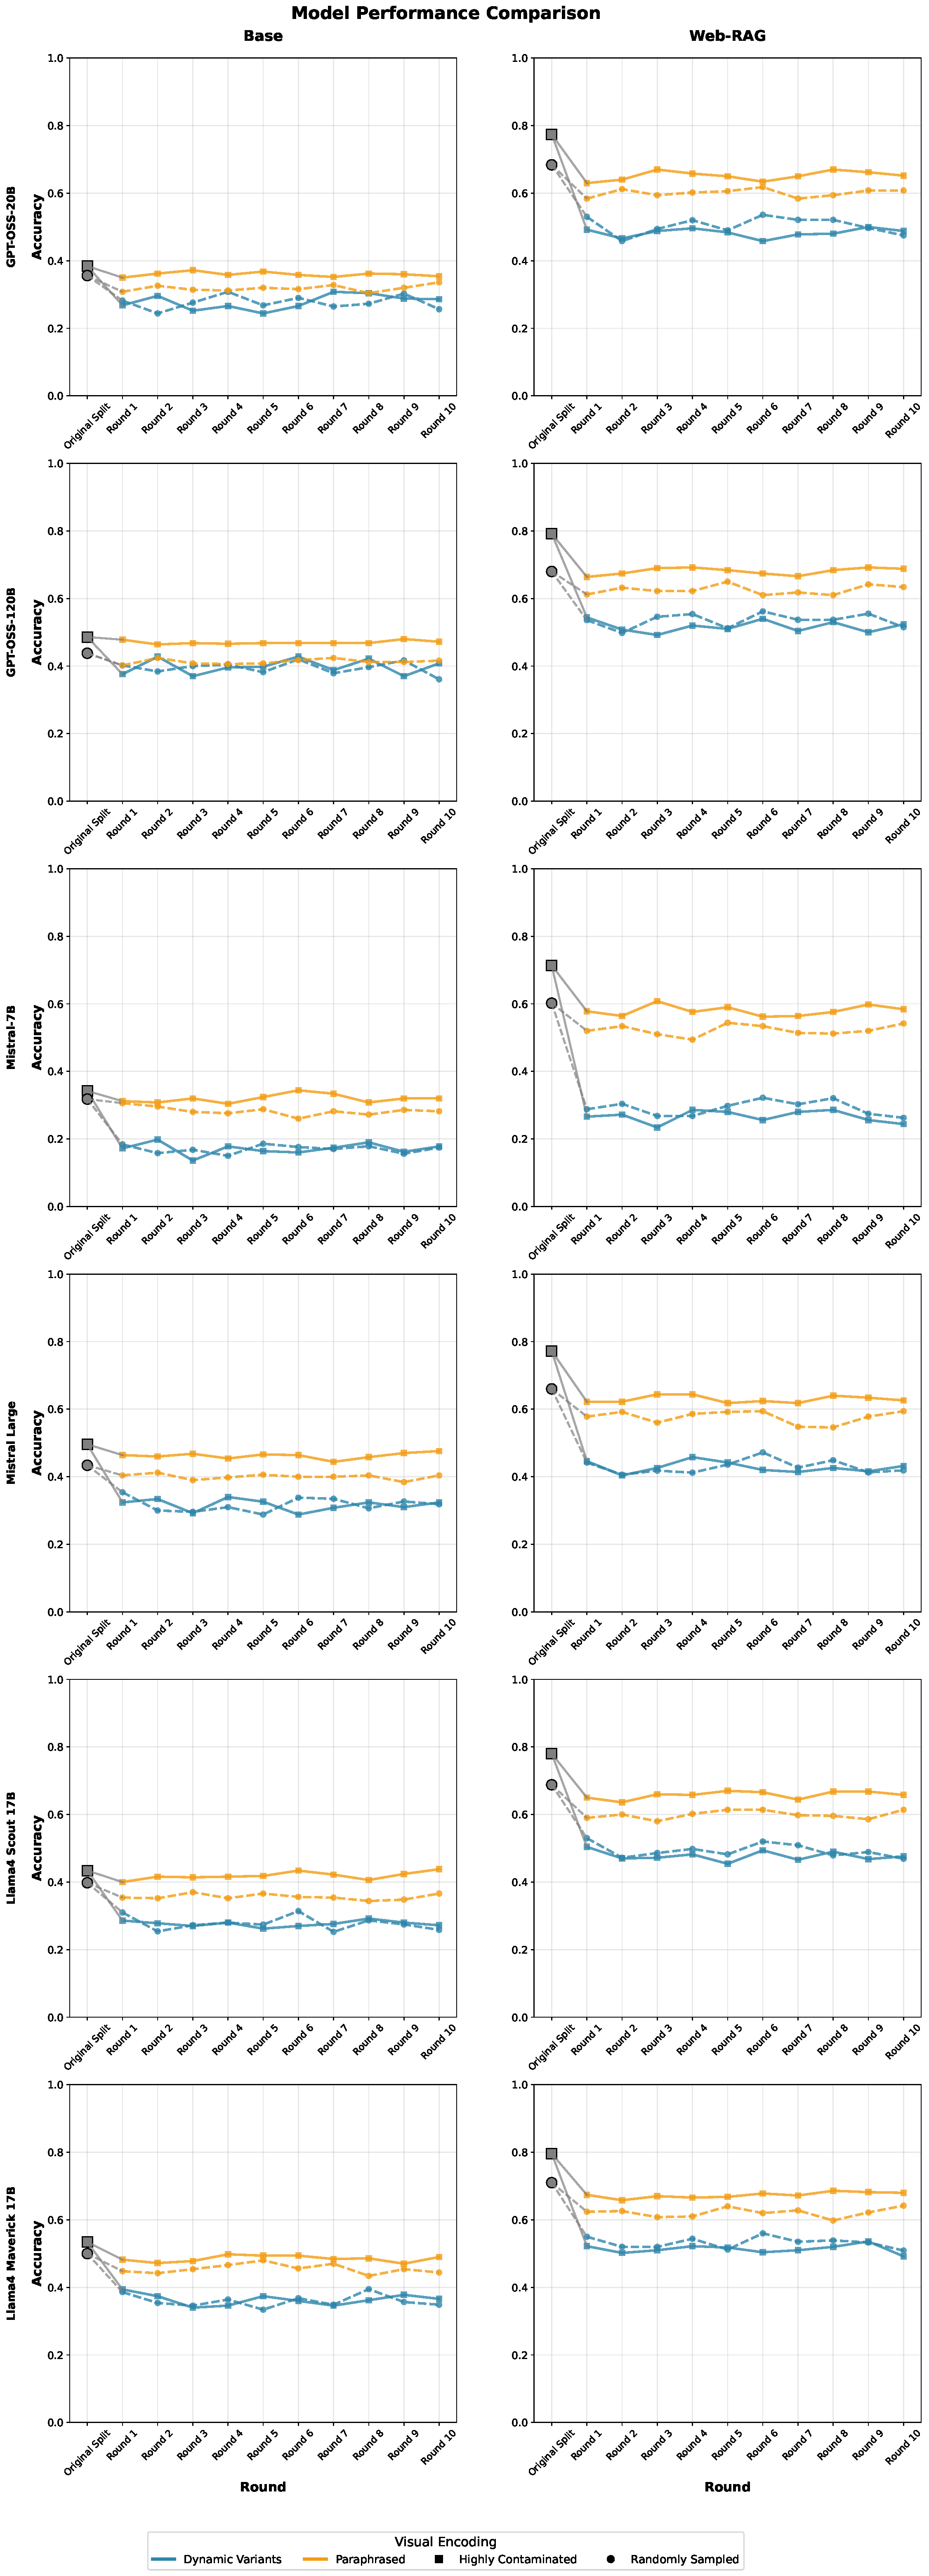
\includegraphics[width=\columnwidth]{res/model_performance_collage.pdf}
    \caption{model\_performance\_collage.pdf}
    \label{fig:model_performance_collage}
\end{figure}

\begin{figure}[htbp]
    \centering
    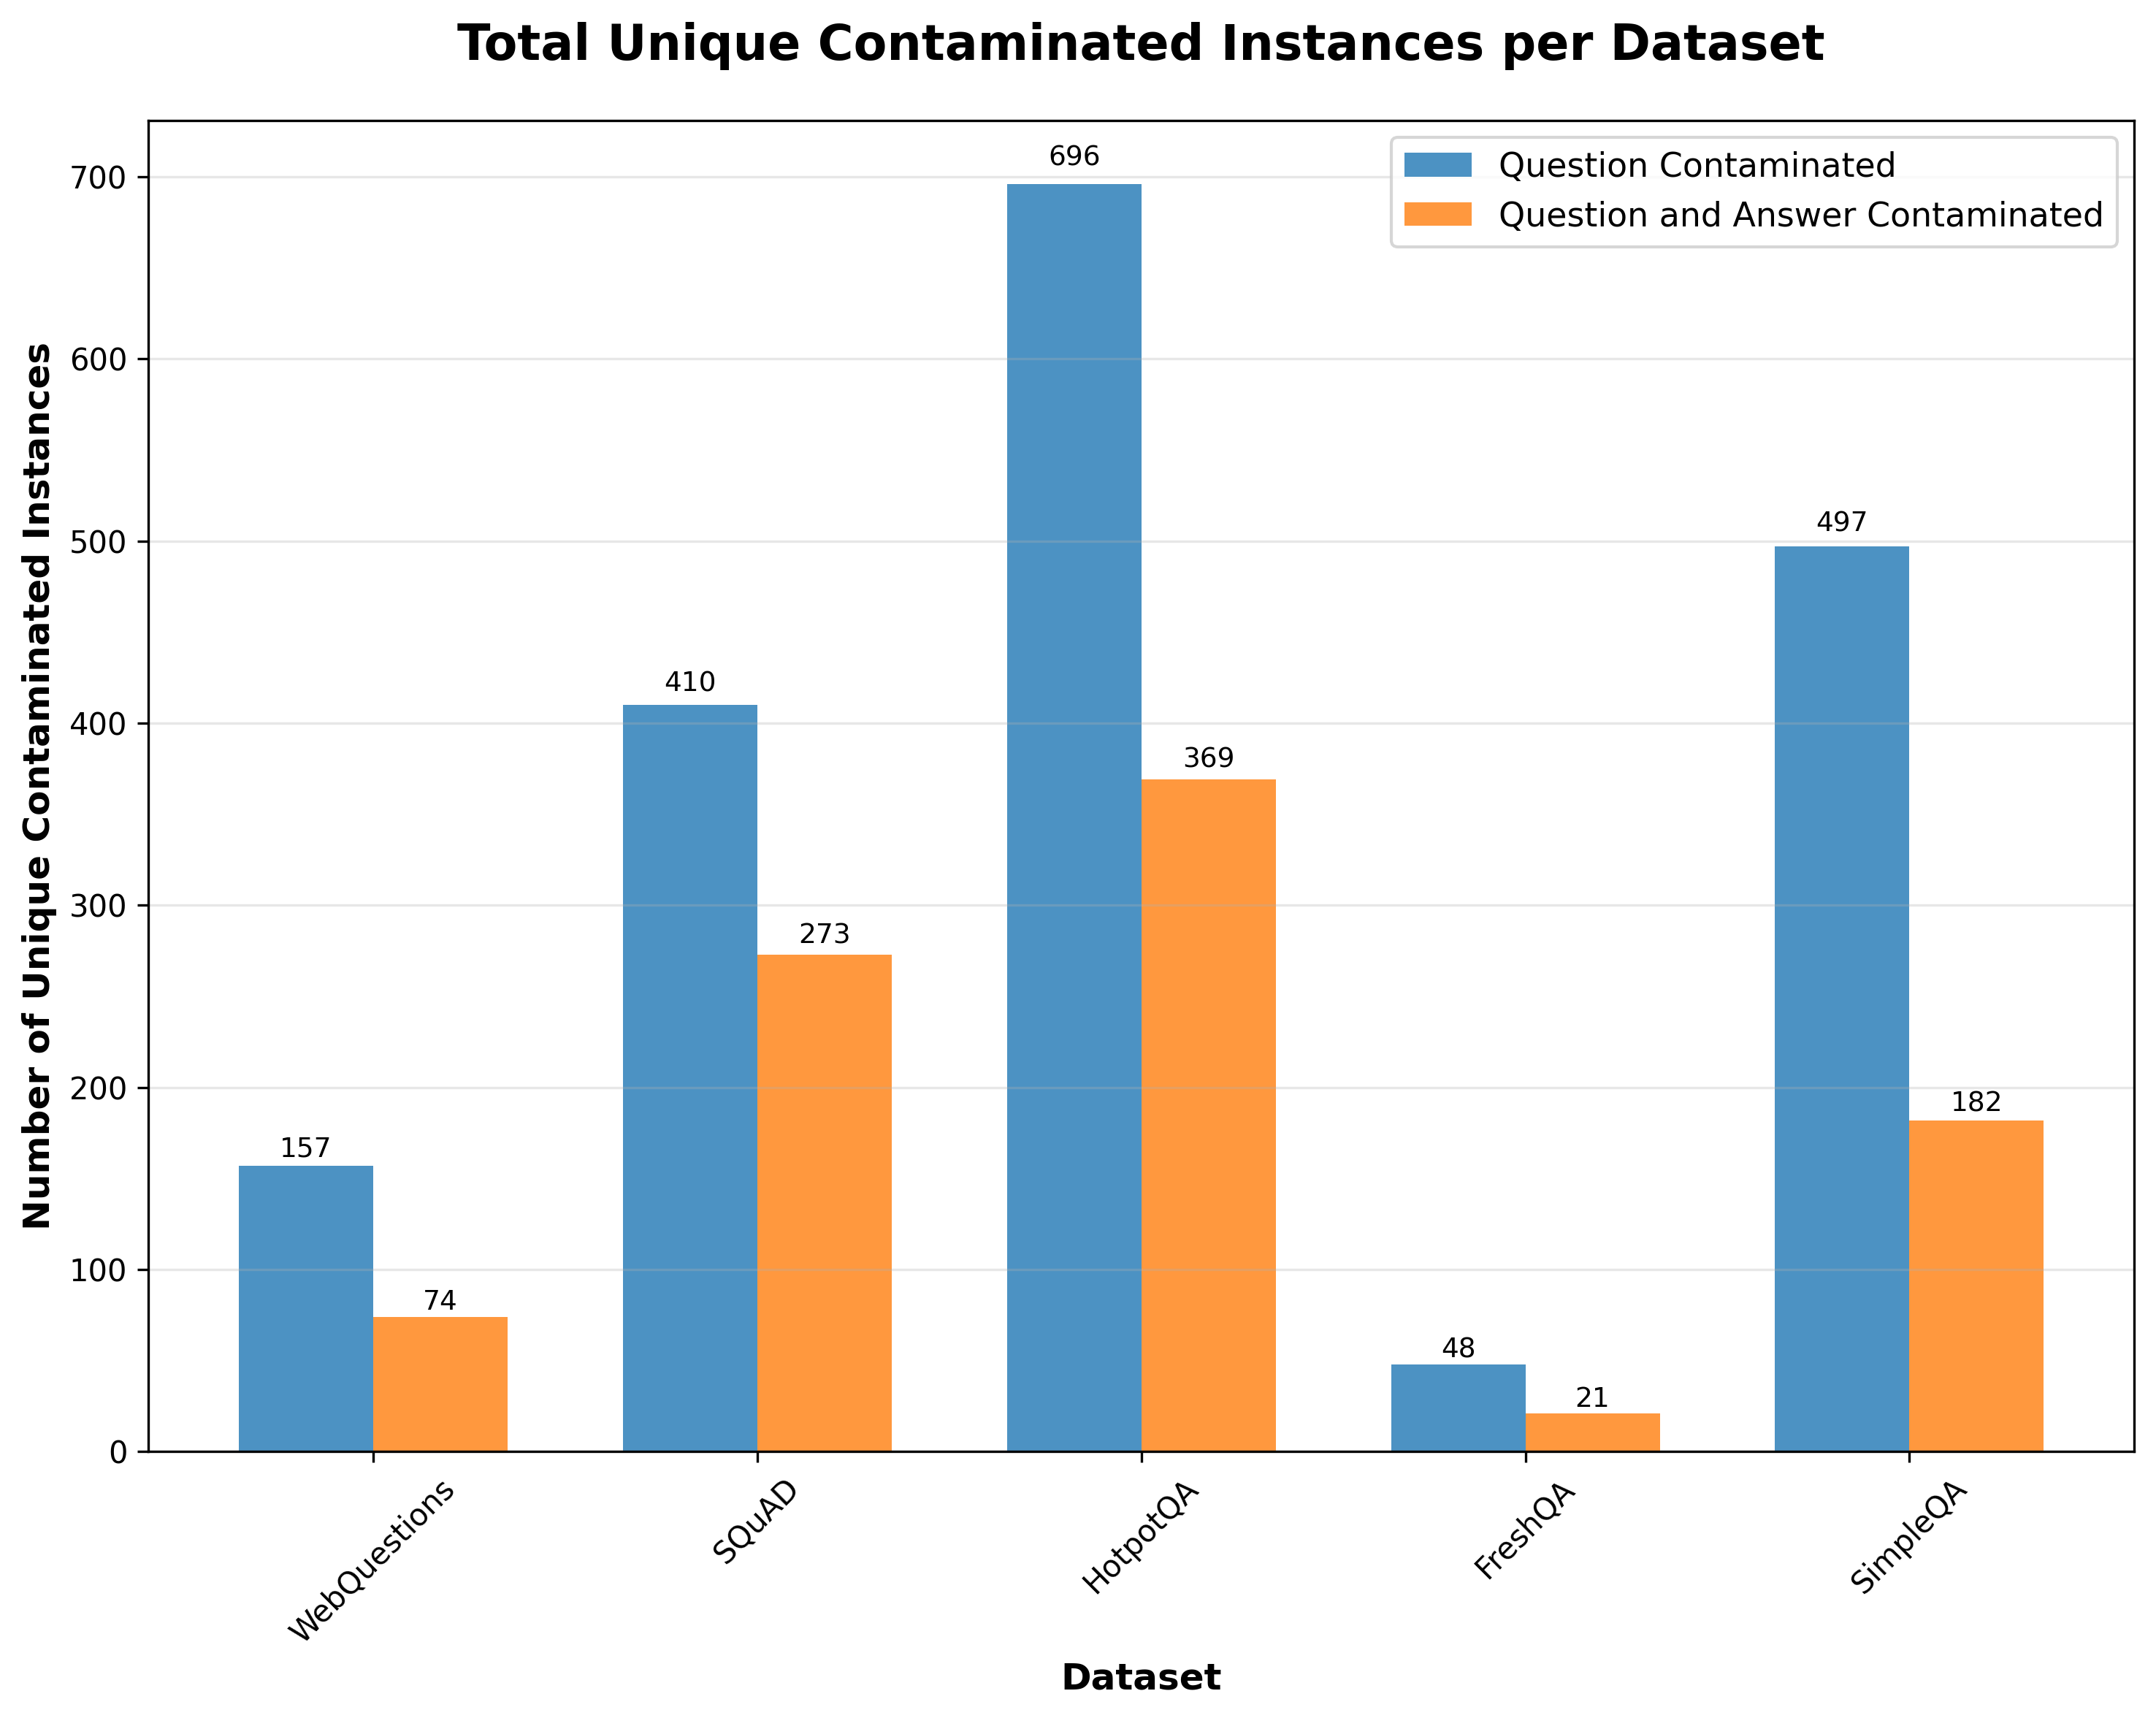
\includegraphics[width=\columnwidth]{res/total_unique_contaminated_instances_per_dataset.png}
    \caption{total\_unique\_contaminated\_instances\_per\_dataset.png}
    \label{fig:total_unique_contaminated_instances}
\end{figure}

\begin{figure}[htbp]
    \centering
    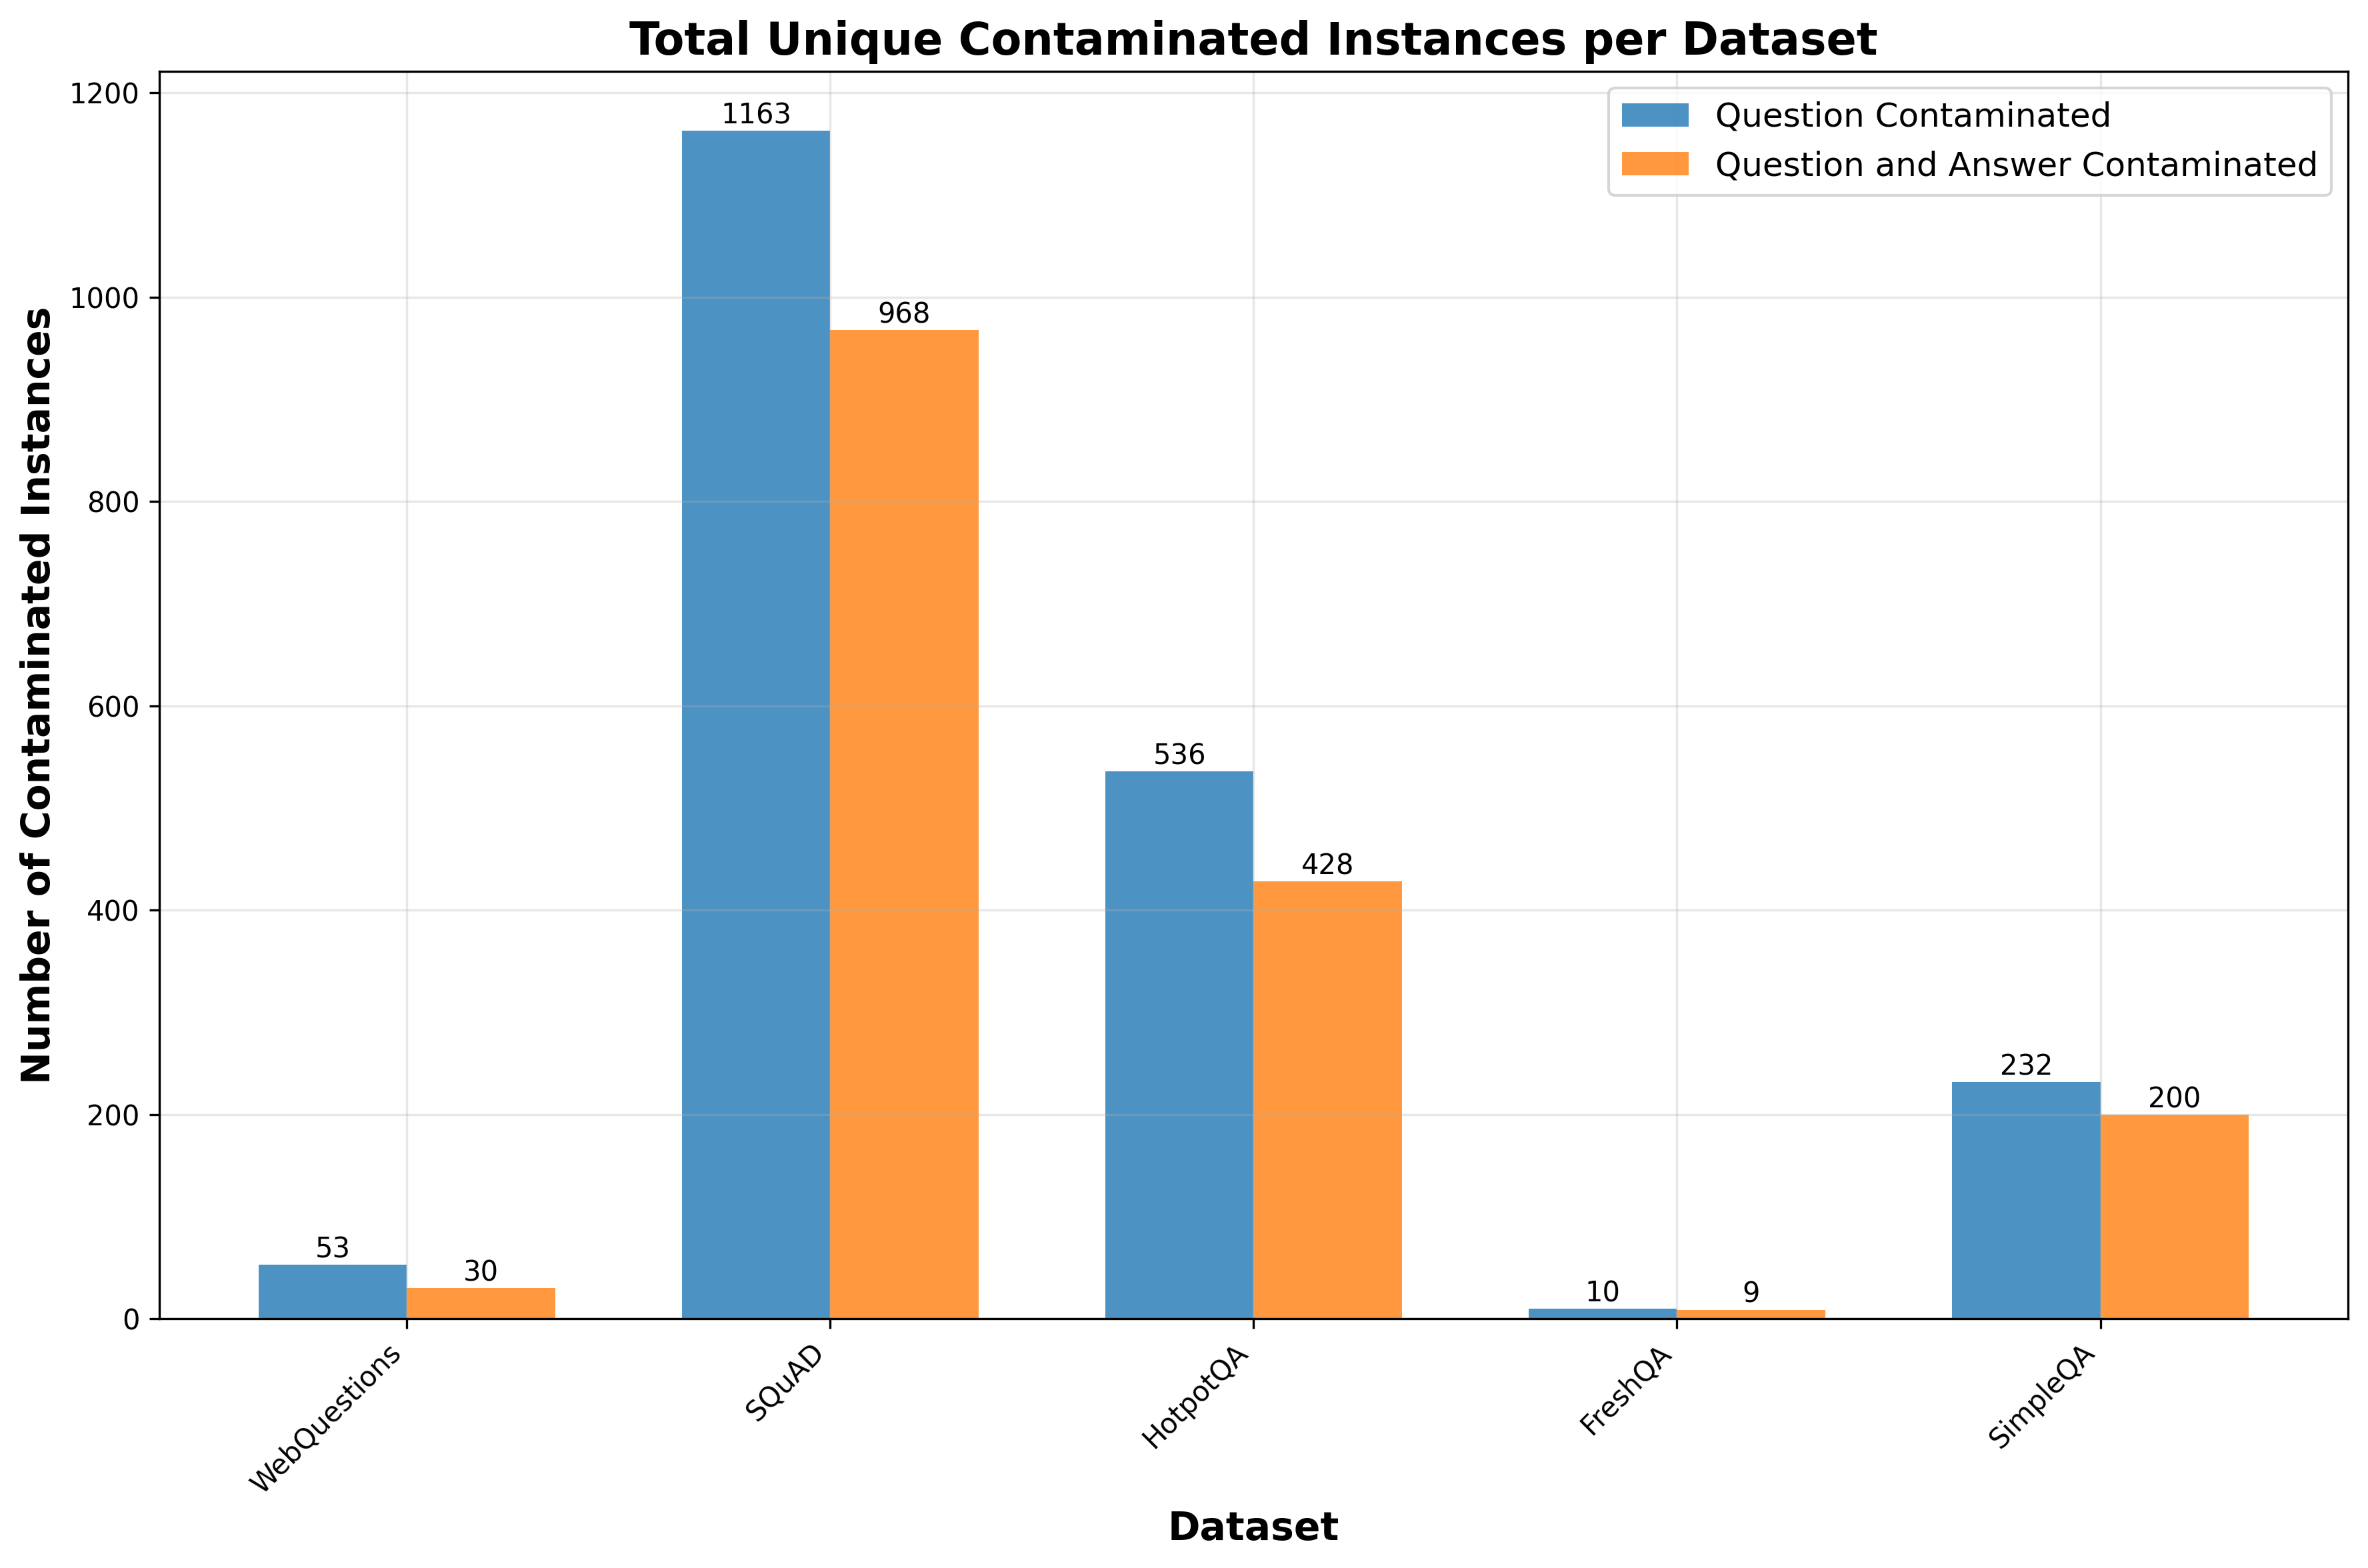
\includegraphics[width=\columnwidth]{res/total_unique_retrieval_contaminated_instances_per_dataset.png}
    \caption{total\_unique\_retrieval\_contaminated\_instances\_per\_dataset.png}
    \label{fig:total_unique_retrieval_contaminated_instances}
\end{figure}

\section{Discussion}
TBD

\section{Conclusion}
TBD


\bibliographystyle{ACM-Reference-Format}
\bibliography{bibliography}

\end{document}
